\chapter{Penetration testing} \label{ch:pentesting}
This chapter details all penetration tests that were performed on the system. These were derived from the threat model created in chapter \ref{ch:threat-model}. All penetration tests are described in the format outlined below. If an aspect of the test was considered simple then one or more parts have been omitted.
\begin{itemize}
    \item \textit{Introduction}. Describes the attack vector that this penetration test will explore.
    \item \textit{Background}. Details the required background knowledge to perform and evaluate this penetration test, if any.
    \item \textit{Method}. Describes in detail how the test was performed, e.g in what environment, with what tools, what commands were used, etc.
    \item \textit{Results}. Describes the findings of the penetration test.
    \item \textit{Discussion}. This section contains a discussion about the reliability, validity, and generalizability of the results.
\end{itemize}

\section{Task 1: Climax Technology's Vesta platform} \label{ch:pentesting:vesta}
Climax Technology, the manufacturer of the hardware used in this system, does not seem to be a consumer-facing business. Nonetheless, they have their own software platform to control their system, called \textit{Vesta}. In the SecuritasHome system, this platform and its components are essentially replaced by \textit{Alarm.com}. The Vesta platform features a mobile application\footnotelink{https://play.google.com/store/apps/details?id=com.climax.vestasmarthome.eu}{2021-04-20} to control the system, as well as a web portal\footnotelink{https://eu.vestasmarthome.com/Vesta/}{2021-04-20}. A potential security vulnerability is if this Vesta platform is still active and usable to control this system.

\subsection{Background}
As stated above, Climax Technology have their own platform, branded as Vesta, to control the system. A common vulnerability in IoT devices is not covering up vulnerabilities arising higher up in the supply chain (\todo source). In this system, there is a possibility that \textit{Alarm.com} has not properly deactivated the access and functionality of the Vesta platform. The idea is for the Alarm.com platform to replace it entirely.

In the app \textit{Vesta Home 5 EU}, see figure \ref{fig:vesta-home-app}, one can perform essentially all actions that the Alarm.com mobile application provides (see section \ref{ch:system:software}). On the landing page, you are greeted with simple a login page (where your Alarm.com credentials don't work). However, it also includes a button labeled \textit{First Time Registration} (see figure \ref{fig:vesta-landing-page}), where one can register a new account connected to a new system. To register a new system one only needs to enter its MAC address, see \ref{fig:vesta-registration-page}, which is available without authorization from the local admin page (see \ref{ch:system:software}). Potentially, one could then register the system in the Vesta platform to gain authorization to control the system, thus bypassing the security completely.
\begin{figure}[!ht]
    \centering
    \begin{subfigure}[t]{0.5\textwidth}
        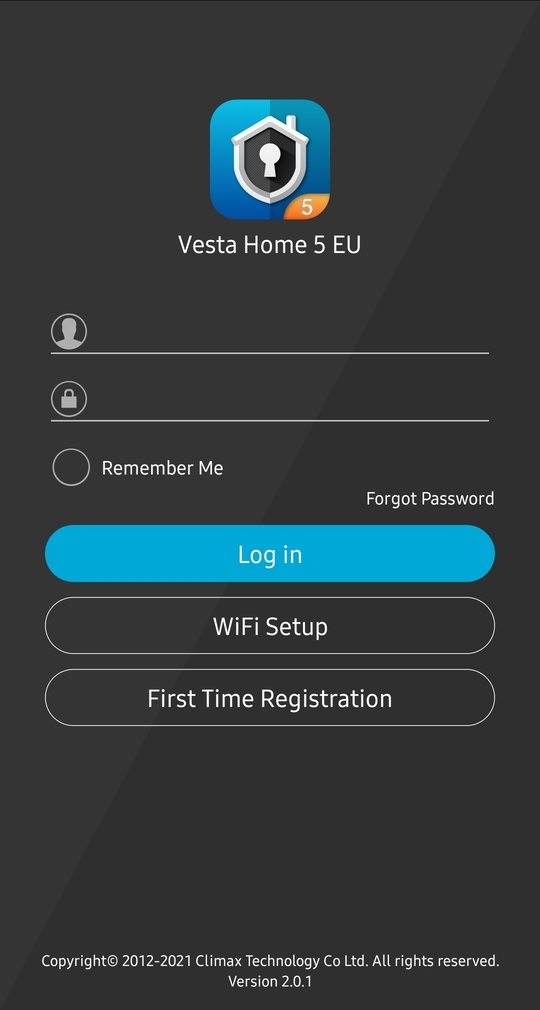
\includegraphics[height=4.8in]{images/6-pentesting/vesta-home-landing-page.jpg}
        \caption{The landing page}
        \label{fig:vesta-landing-page}
    \end{subfigure}%
    ~
    \begin{subfigure}[t]{0.5\textwidth}
        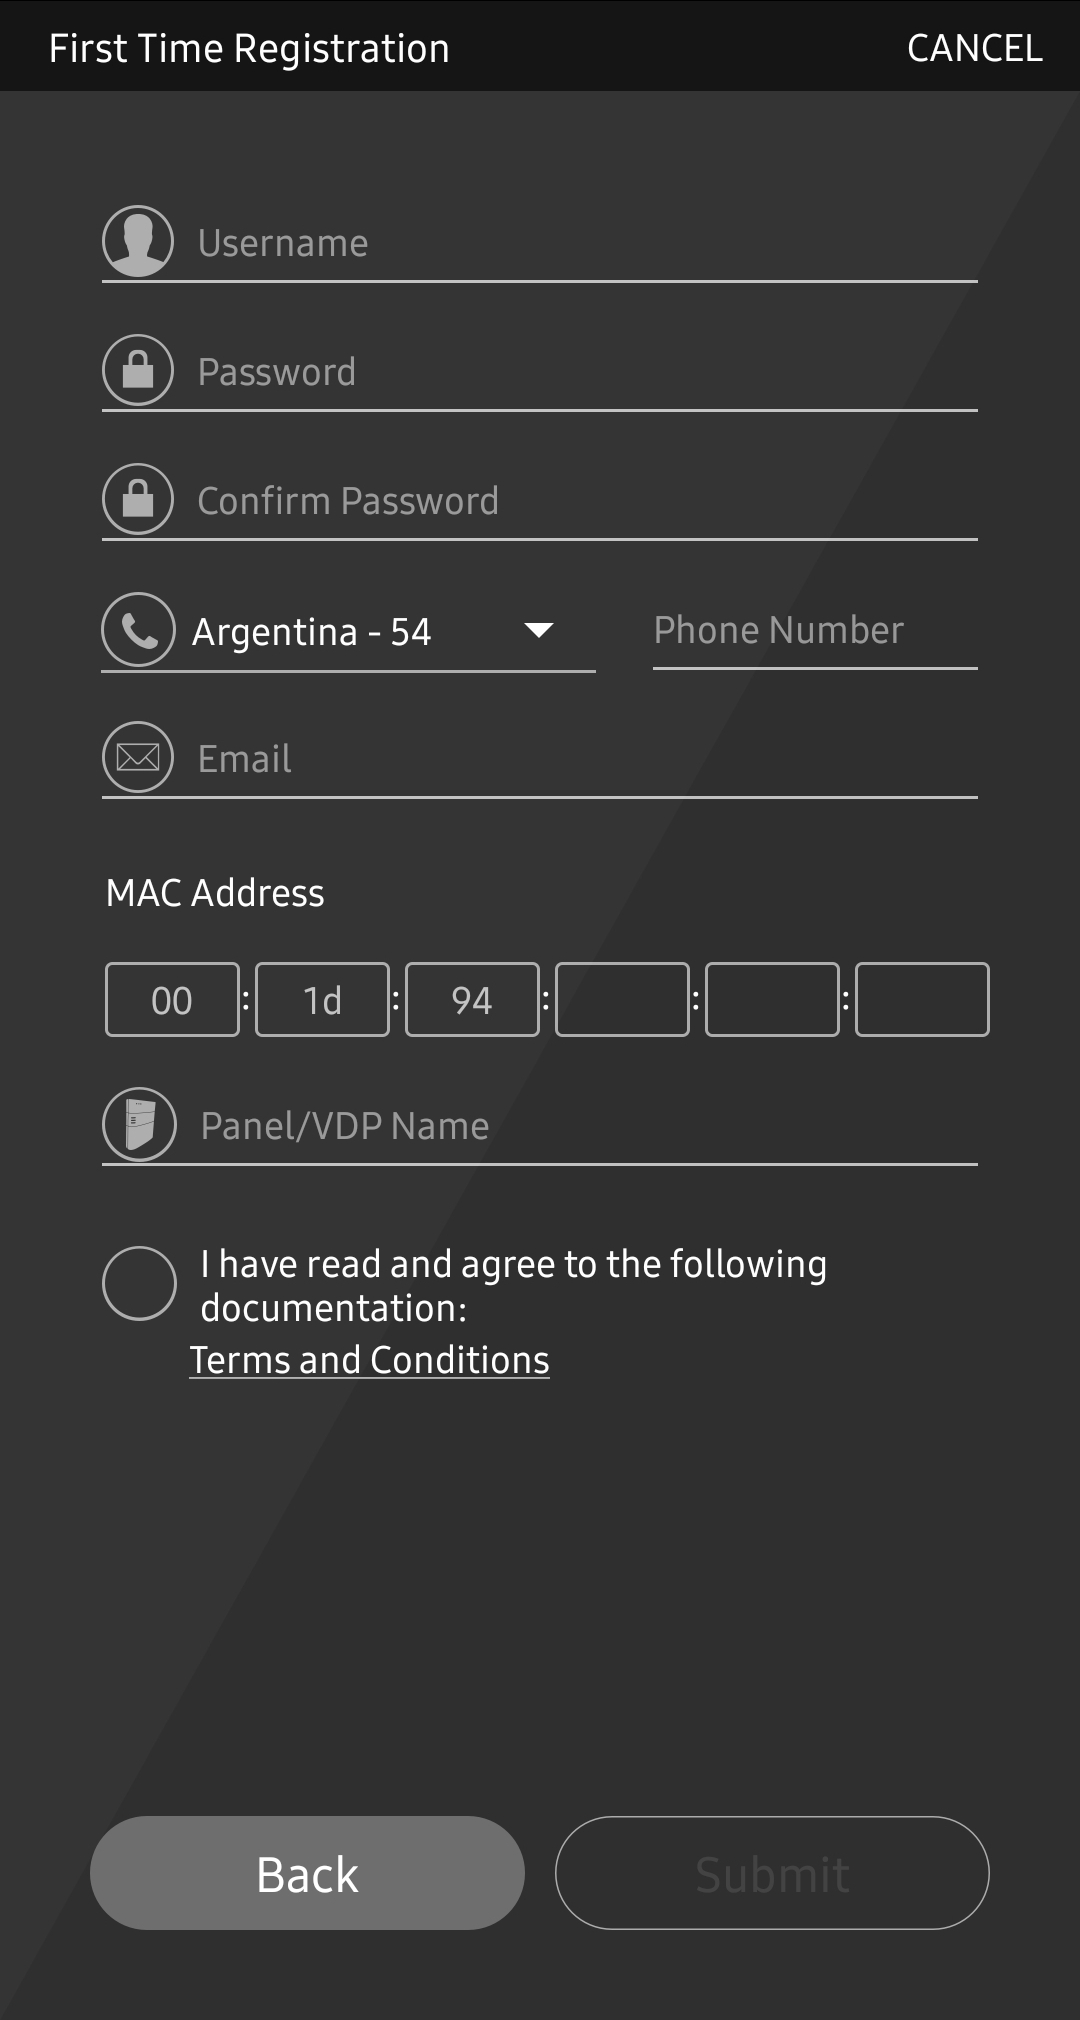
\includegraphics[height=4.8in]{images/6-pentesting/vesta-home-registration.jpg}
        \caption{The "First Time Registration" page}
        \label{fig:vesta-registration-page}
    \end{subfigure}
    \caption{The Vesta Home 5 EU mobile application.}
    \label{fig:vesta-home-app}
\end{figure}
In the Vesta web application, there is a very similar form, allowing you to register a new device using the MAC address, see figure \ref{fig:vesta-web-registration}.
\begin{figure}[!ht]
    \centering
    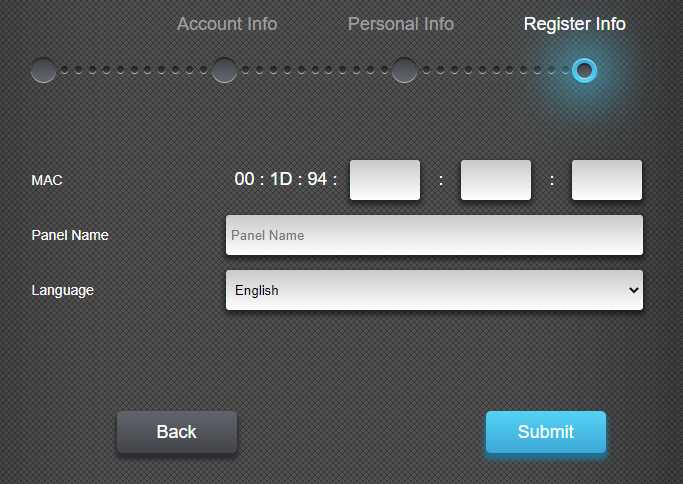
\includegraphics[width=\textwidth]{images/6-pentesting/vesta-web-registration.png}
    \caption{The Vesta web application registration.}
    \label{fig:vesta-web-registration}
\end{figure}

\subsection{Method}
The mobile application is free to download. To be able to confidently monitor the network traffic, the mobile application was installed on an android emulator for PC, and Wireshark was run on the host machine. Both applications use HTTPS, meaning the requests are encrypted.

An attempt was made to perform a \gls{MITM} attack on the mobile application to view the HTTPS traffic, using \textit{mitmproxy}\footnotelink{https://mitmproxy.org/}{2021-04-21} and the built-in proxy settings of the android emulator. However, this made the application yield an error message saying it could not reach the server. Presumably, the application uses certification pinning to protect against this type of attack. This was not explored further since the traffic can easily be viewed in the web application, using the Chrome network tab (see figure \ref{fig:vesta-web-registration-failed}), and most likely both applications access the same API.

\subsection{Results}
The penetration test was unsuccessful. Both the mobile application and the web application yielded identical results. A simple error message is shown, saying the \textit{MAC/IMEI} is incorrect, see figures \ref{fig:vesta-home-registration-failed} and \ref{fig:vesta-web-registration-failed}. In the Chrome network tab, we can see when trying to register the system through the web application that the API responds with the message "no data found!".
\begin{figure}[!ht]
    \centering
    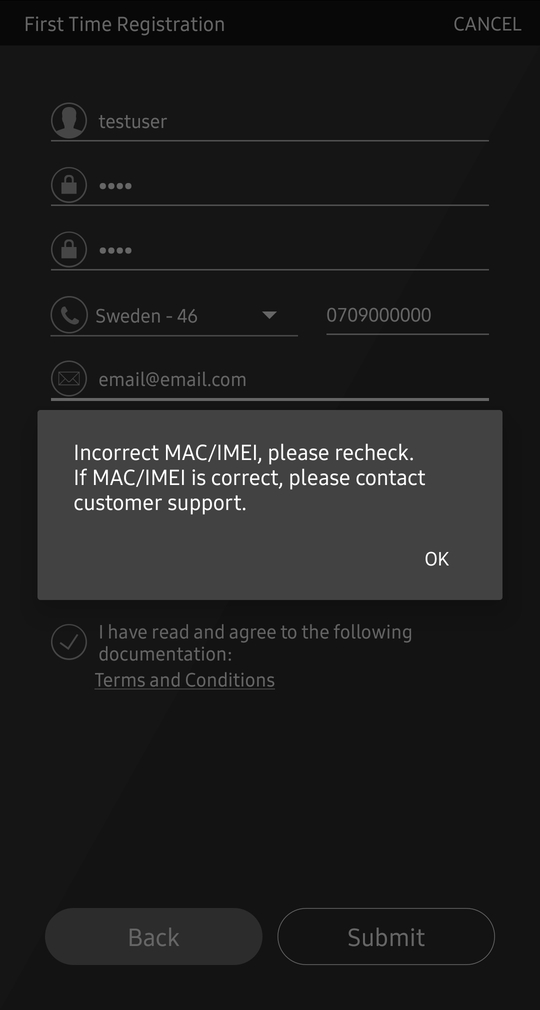
\includegraphics[width=0.5\textwidth]{images/6-pentesting/vesta-home-registration-failed.jpg}
    \caption{The results of trying to register in the mobile app.}
    \label{fig:vesta-home-registration-failed}
\end{figure}
\begin{figure}[!ht]
    \centering
    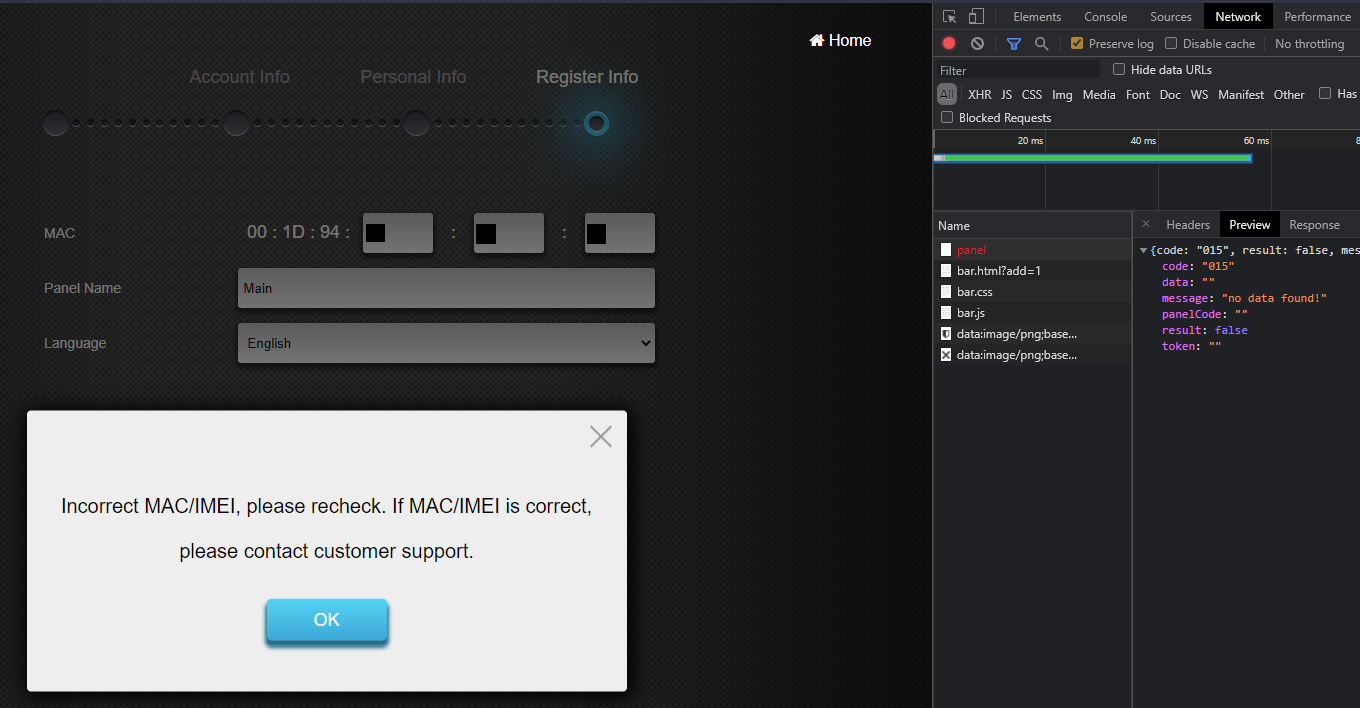
\includegraphics[width=\textwidth]{images/6-pentesting/vesta-web-registration-failed.png}
    \caption{The results of trying to register in the web app.}
    \label{fig:vesta-web-registration-failed}
\end{figure}

\subsection{Discussion}
Trying to register the hardware to the Vesta platform was unsuccessful. The given MAC address was not accepted. Presumably, Climax Technology has a database of the MAC addresses of all sold systems under the Vesta platform. While the MAC address of the system in this thesis is registered under Climax Technology, it does not seem to be registered by the Vesta platform. Another possibility is that the MAC address and IMEI number pair is not registered because \textit{Alarm.com} has used their own SIM cards and thus a different IMEI number. This is indicated by the error messages shown. Which of these scenarios is the correct one, we cannot know. Either way, we can see that the API responds with a negative result, saying that no data could be found. Therefore, this type of supply chain error seems to have been identified and correctly protected against.

\section{Task 2: Online Password Attack}
An online password attack refers to probing an active login, as opposed to an offline attack where you for example might try to crack a hash of a leaked database. This attack involves using some type of approach to test many passwords of a login form to try and find valid credentials. The local web admin page (see section \ref{ch:system}) has a login page that could potentially be brute-forced.

\subsection{Background}
A password attack, or password cracking, refers to cyber-attacks where the attacker tries to figure out valid credentials, to gain authorized access to a system. These can be categorized into two groups: offline and online password attacks. The former refers to attacks requiring no communication with the system in order to test a valid password. An example could be listening in on network traffic and seeing a password hash. One could then perform an offline password attack by trying to figure out which password produced that hash, and thus login to the system. In an online attack, the system under attack is in continuous communication with the attacker. This could be, for example, writing a script to try many different passwords on a login page of a web page. Online password attacks are generally harder to successfully perform. They are often much slower, as the communication with the system incurs a major overhead, and also poses the potential risk of getting caught in the middle of it if the administrator of the system notices the malicious traffic. Servers also often implement rate-limiting against IP addresses to combat these types of attacks.

For both online and offline password attacks, there are several techniques one can use to try and guess the correct password. The simplest one is a \textit{brute-force attack}, where the attacker simply tries all possible passwords up to some length. Given $c$ possible characters in the password and a password length of $l$, there are $c^l$ possible passwords to try. This has exponential complexity in the length of the password, and will thus scale very poorly with longer passwords. Another technique is called a \textit{dictionary attack}, where the attacker uses a large list of known common passwords. Often these lists are created from actual passwords from leaked databases. For offline attacks like hash-cracking, there are additional techniques like \textit{rainbow tables}.

In the case of the system in this thesis, we have no opportunity for an offline password attack, as no information about the password such as a hash is leaked as far as the author is aware. The local admin web page does, however, feature a login page. This page uses \textit{HTTP Basic authentication} to log in to the main panel (see figure \ref{fig:local-login-page}). If this login system has not implemented any form of rate-limiting then guessing the right password might be possible, given enough time and resources.

\subsection{Method}
We know from sources like the one covered in section \ref{ch:related-work:lupus} that \textit{admin} is most likely a valid user name. This is further indicated by the official user manual from Climax Technology\footnotelink{https://fccid.io/GX9HSGWF1919/Users-Manual/Users-Manual-4873123}{2021-04-22}, which includes default login credentials with the admin user name (the credentials do not work on this system). As stated, the login form (see figure \ref{fig:local-login-page}) uses \textit{HTTP Basic authentication} to authenticate the user. A dictionary attack was performed against this login page. The well-known password list \textit{rockyou.txt} was used as the dictionary. A useful tool to perform online password attacks is called \textit{Hydra}\footnotelink{https://github.com/vanhauser-thc/thc-hydra}{2021-04-21}, which is a command-line tool. Using the following command, Hydra was used to perform the attack:
\begin{lstlisting}[frame=tb]
    hydra -l admin       \
          -P rockyou.txt \
          192.160.1.90   \
          http-get       \
          "/action/login:A=BASIC:F=Access Denied"
\end{lstlisting}

\subsection{Results}
The test was mostly unsuccessful. A password attack against the system was successfully completed. However, Hydra only manages to perform around 23 requests per minute against the main panel, see figure \ref{fig:hydra-password-attack}. This is too slow to be able to guess enough passwords to have a meaningful probability at a correct guess.
\begin{figure}[!ht]
    \centering
    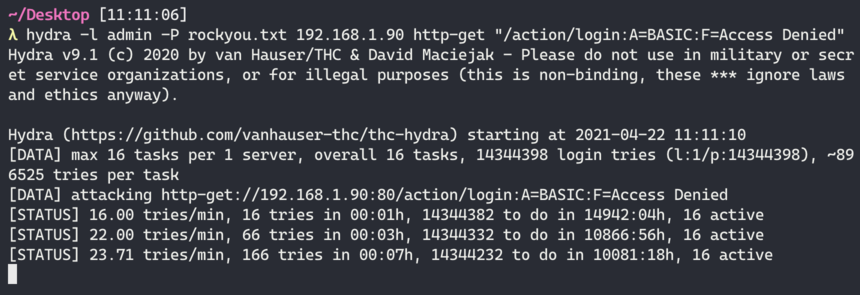
\includegraphics[width=\textwidth]{images/6-pentesting/hydra-results.png}
    \caption{The results of running a password attack.}
    \label{fig:hydra-password-attack}
\end{figure}

\subsection{Discussion}
The Hydra tool was only able to do around 23 requests per minute. Hydra is known to be very fast, so that is not the issue. One explanation for why this was so slow could be that the server rate-limits users. This is a common technique to protect against password attacks, if enough failed login attempts occur from a single IP the server would temporarily block it or slow down the response time. However, there are signs indicating that this is not the case. For example, accessing the main web page slows down tremendously while performing the attack. Initially, it had around a \textit{16ms} response time, which increased to about \textit{17 seconds} during the attack. This was even confirmed on another computer, indicating that the main panel has not implemented any form rate-limiting per IP address. Presumably, the system is instead simply resource-bound and cannot serve requests at a faster rate. Given the hardware of the system, this is not unlikely. The CPU is most likely not that powerful, as is often the case in \gls{IOT} systems.

Due to the main panel not being able to serve more than 23 requests per minute, this type of attack is not feasible. For example, running a brute force attack, testing just all possible eight-character passwords, would take well over a hundred thousand years. A well-crafted dictionary attack could perhaps be effective, even at these slow speeds. However, there is some indication that the password might be just a random string of characters, given that the default password cited in the user manual is \texttt{cX+HsA*7F1}. If that is the case then a brute force technique is the only possibility. For these reasons, the attack was deemed unfeasible and not pursued further.
